Section \ref{sec:summary-nts-mtds} highlights the poor performance of neutron diffusion
methods for calculating neutron fluxes near control rods. Strong neutron absorption in the control
rod region produces a highly anisotropic neutron flux extending some distance outside the control
rod. Neutron transport methods, which retain angular dependence of the neutron flux to various
extents, generally fare better than neutron diffusion methods, which have isotropic diffusion
coefficients. However, neutron transport methods are also generally more computationally expensive,
given the increased dimensionality of the problem from the angular component. Adding an angular
dimension to the existing geometric and neutron energy group dimensions dramatically
increases the problem size and the computational resources necessary to solve the system. Many past
efforts have tried introducing
transport correction techniques to improve neutron flux and multiplication factor estimates in
diffusion-based methods. Other than control rod regions, these techniques may also correct
homogenization errors introduced by spatial homogenization of fuel assemblies and other
structures within a reactor core. They invariably rely on neutron transport methods to generate
transport corrections in the form of corrected diffusion coefficients
\cite{bretscher_computing_1997, scherer_determination_1976, ronen_accurate_2004,
pounders_diffusion_2009, kavenoky_sph_1978}, boundary conditions \cite{davison_influence_1951,
pellaud_extrapolation_1968, fen_modelling_1992}, Eddington factors, or discontinuity factors
\cite{koebke_new_1980}.

In this chapter, I propose a hybrid $S_N$-diffusion neutronics method to improve control rod
modeling in neutron diffusion solvers without spatial homogenization. In essence, the hybrid
method is an iterative method that applies
the $S_N$ discrete ordinates neutron transport method on subregions containing the control rod to
obtain pointwise transport corrections for the diffusion method on the subregions.
This chapter presents the mathematical derivation for the
\gls{SAAF} formulation of the $S_N$ equations and the drift transport correction term for the
neutron diffusion equations, and the computational algorithm for the hybrid method.

Section \ref{sec:saaf} provides the mathematical derivation for the discretized weak form of the
\gls{SAAF} $S_N$ neutron transport equations. Section \ref{sec:transport-correction} provides the
derivations for the transport correction formulations I investigated for use in the hybrid method.
Section \ref{sec:hybrid-algorithm} details the iteration algorithm for the hybrid method. Section
\ref{sec:sn-bc} provides the boundary conditions formulated for the $S_N$ calculations in the
hybrid method. In Section \ref{sec:buffer-region}, I discuss how transport corrections are handled
in the hybrid method. Lastly, Section \ref{sec:hybrid-summary} summarizes the hybrid method and its
implementation.

% Section \ref{sec:theory} discusses the theoretical background for the hybrid $S_N$-diffusion
% method. Section \ref{sec:implementation} provides numerical implementation details of
% the hybrid method and its components. Sections \ref{sec:test-case} and \ref{sec:sim-param} describe
% the 1-D test cases and several simulation parameters in that context. Section
% \ref{sec:prelim-results} discusses the results of the hybrid method applied to the 1-D test cases
% with comparisons to higher-fidelity Monte Carlo and $S_N$ neutron transport methods. Lastly,
% Section \ref{sec:hybrid-summary} summarizes the key findings in this chapter.

\section{\Gls{SAAF} $S_N$ Method} \label{sec:saaf}

This chapter starts with the $S_N$ method implementation required for the hybrid $S_N$-diffusion
method. I implemented both $S_N$ and hybrid methods using \gls{FEM} numerical solver capabilities
available through Moltres \cite{lindsay_moltres_2017} and the \gls{MOOSE} framework. In this
section, the derivation for the \gls{SAAF} formulation of the $S_N$ method and its
implementation in Moltres follows closely the derivation developed by Wang et al.\
\cite{wang_diffusion_2014, wang_rattlesnake_2018}.

\subsection{Multigroup Neutron Transport Equations}

Continuing from the introduction to neutronics methods in Section \ref{sec:summary-nts-mtds},
the time-dependent, multigroup neutron transport equation defined on the 3-D spatial domain
$\mathcal{D}$ and 2-D unit sphere angular domain $\mathcal{S}$ is:
%
\begin{multline}
  \frac{\partial}{\partial t}\left[\frac{\Psi_g(\vec{r},\hat{\Omega},t)}{v_g}\right] +
  \hat{\Omega}\cdot\nabla\Psi_g(\vec{r},\hat{\Omega},t) + \Sigma_{t,g}
  \Psi_g(\vec{r},\hat{\Omega},t) =
  \sum^G_{g'=1}\int_\mathcal{S} \Sigma_s^{g'\rightarrow g}(\hat{\Omega}'\rightarrow\hat{\Omega})
  \Psi_{g'}(\vec{r},\hat{\Omega}',t)d\hat{\Omega}' \\
  + \frac{1}{4\pi}\chi_{p,g}(1-\beta)\sum^G_{g'=1} \nu\Sigma_{f,g'} \phi_{g'}(\vec{r},t)
  + \frac{1}{4\pi}\sum^I_{i=1}\chi_{d,g}
  \lambda_i C_i(\vec{r},t) + Q^{\text{ext}}_g(\vec{r},\hat{\Omega})
  \label{eq:mg-nte}
\end{multline}
%
with the boundary conditions
%
\begin{gather}
  \Psi_g(\vec{r},\hat{\Omega}) = \Psi^\text{inc}_g(\vec{r},\hat{\Omega}) +
  \alpha^s_g\Psi_g(\vec{r},\hat{\Omega}_r)
  \mbox{ on } \vec{r} \in \partial\mathcal{D} \mbox{ and } \hat{\Omega}\cdot\hat{n}_b < 0,
  \shortintertext{where}
  \begin{align*}
    \chi_{p,g} &= \mbox{prompt fission neutron spectrum in group $g$,} \\
    \beta &= \sum^I_{i=1} \beta_i = \mbox{total delayed neutron fraction,} \\
    \chi_{d,g} &= \mbox{delayed fission neutron spectrum in group $g$,} \\
    \lambda_i &= \mbox{decay constant of precursor group $i$,} \\
    C_i &= \mbox{delayed neutron precursor concentration for group $i$,} \\
    \Psi^\text{inc}_g &= \mbox{incident surface source in group $g$,} \\
    \alpha^s_g &= \mbox{specular reflectivity on }\partial \mathcal{D} \mbox{ for group }g, \\
    \hat{\Omega}_r &= \hat{\Omega}-2(\hat{\Omega}\cdot \hat{n}_b)\hat{n}_b, \\
    \hat{n}_b &= \mbox{outward unit normal vector on the boundary.}
  \end{align*}
\end{gather}
%
In order to introduce operators and facilitate subsequent mathematical derivations, we will define
the following vector forms:
%
\begin{gather}
  \bm{\Psi} \equiv
  \begin{bmatrix}
    \Psi_1 \\
    \Psi_2 \\
    \vdots \\
    \Psi_G
  \end{bmatrix},
  \bm{\Phi} \equiv \int_S \bm{\Psi}d\hat{\Omega} \equiv
  \begin{bmatrix}
    \phi_1 \\
    \phi_2 \\
    \vdots \\
    \phi_G
  \end{bmatrix},
  \bm{\frac{\Psi}{v}} \equiv
  \begin{bmatrix}
    \frac{\Psi_1}{v_1} \\
    \frac{\Psi_2}{v_2} \\
    \vdots \\
    \frac{\Psi_G}{v_G}
  \end{bmatrix},
  \bm{C} \equiv
  \begin{bmatrix}
    C_1 \\
    C_2 \\
    \vdots \\
    C_G
  \end{bmatrix},
  \bm{Q}^{\text{ext}} \equiv
  \begin{bmatrix}
    Q^\text{ext}_1 \\
    Q^\text{ext}_2 \\
    \vdots \\
    Q^\text{ext}_G
  \end{bmatrix}, \nonumber
%  \bm{Q}_f = \frac{1}{4\pi}\bm{Q}_{f,0} =
%  \begin{bmatrix}
%    \frac{1}{4\pi}\chi_{p,1}(1-\beta)\sum^G_{g'=1} \nu\Sigma_{f,g'} \phi_{g'} +
%    \frac{1}{4\pi}\sum^I_{i=1}\chi_{d,1} \lambda_i C_i \\
%    \frac{1}{4\pi}\chi_{p,2}(1-\beta)\sum^G_{g'=1} \nu\Sigma_{f,g'} \phi_{g'} +
%    \frac{1}{4\pi}\sum^I_{i=1}\chi_{d,2} \lambda_i C_i \\
%    \vdots \\
%    \frac{1}{4\pi}\chi_{p,G}(1-\beta)\sum^G_{g'=1} \nu\Sigma_{f,g'} \phi_{g'} +
%    \frac{1}{4\pi}\sum^I_{i=1}\chi_{d,G} \lambda_i C_i
%  \end{bmatrix},
%  \bm{Q} = \bm{Q}_f + \bm{Q}^\text{ext}. \nonumber
\end{gather}
%
We also define the following operators:
%
\begin{gather}
  \mathbb{L}_1\bm{\Psi} \equiv
  \begin{bmatrix}
    \hat{\Omega}\cdot\nabla\Psi_1 \\
    \hat{\Omega}\cdot\nabla\Psi_2 \\
    \vdots \\
    \hat{\Omega}\cdot\nabla\Psi_G \\
  \end{bmatrix},
  \mathbb{L}_2\bm{\Psi} \equiv
  \begin{bmatrix}
    \Sigma_{t,1}\Psi_1 \\
    \Sigma_{t,2}\Psi_2 \\
    \vdots \\
    \Sigma_{t,G}\Psi_G
  \end{bmatrix},
  \mathbb{L}\bm{\Psi} \equiv \mathbb{L}_1\bm{\Psi} + \mathbb{L}_2\bm{\Psi}, \nonumber \\
  \mathbb{S}\bm{\Psi} \equiv
  \begin{bmatrix}
    \sum^G_{g'=1}\int_S \Sigma_s^{g'\rightarrow 1}\Psi_{g'}d\hat{\Omega} \\
    \sum^G_{g'=2}\int_S \Sigma_s^{g'\rightarrow 2}\Psi_{g'}d\hat{\Omega} \\
    \vdots \\
    \sum^G_{g'=G}\int_S \Sigma_s^{g'\rightarrow G}\Psi_{g'}d\hat{\Omega}
  \end{bmatrix},
  \mathbb{B}\bm{\Psi} \equiv
  \begin{bmatrix}
    \alpha^s_1\Psi_1(\hat{\Omega}_r) \\
    \alpha^s_2\Psi_2(\hat{\Omega}_r) \\
    \vdots \\
    \alpha^s_G\Psi_G(\hat{\Omega}_r)
  \end{bmatrix}, \nonumber \\
  \mathbb{F}\bm{\Psi} \equiv \frac{1}{4\pi}\mathbb{F}_0\bm{\Psi} \equiv
  \begin{bmatrix}
    \frac{1}{4\pi}\chi_{p,1}(1-\beta)\sum^G_{g'=1}\nu\Sigma_{f,g'}\phi_{g'} \\
    \frac{1}{4\pi}\chi_{p,2}(1-\beta)\sum^G_{g'=1}\nu\Sigma_{f,g'}\phi_{g'} \\
    \vdots \\
    \frac{1}{4\pi}\chi_{p,G}(1-\beta)\sum^G_{g'=1}\nu\Sigma_{f,g'}\phi_{g'}
  \end{bmatrix},
  \mathbb{C}\bm{C} \equiv \frac{1}{4\pi}\mathbb{C}_0\bm{C} \equiv
  \begin{bmatrix}
    \frac{1}{4\pi}\sum^I_{i=1}\chi_{d,1} \lambda_i C_i \\
    \frac{1}{4\pi}\sum^I_{i=1}\chi_{d,2} \lambda_i C_i \\
    \vdots \\
    \frac{1}{4\pi}\sum^I_{i=1}\chi_{d,G} \lambda_i C_i
  \end{bmatrix}. \nonumber
\end{gather}
%
Note that the operators apply element-wise multiplication as opposed to the more conventional
matrix multiplication. Eq.\ \ref{eq:mg-nte} can be reexpressed as:
%
\begin{gather}
  \frac{\partial}{\partial t} \left(\frac{\bm{\Psi}}{\bm{v}}\right)+\mathbb{L}\bm{\Psi}
  = \mathbb{S}\bm{\Psi} + \bm{Q}, \label{eq:nte-vec}
\end{gather}
%
with the boundary conditions on $\partial\mathcal{D}$
%
\begin{gather}
  \bm{\Psi} = \bm{\Psi}^\text{inc} + \mathbb{B}\bm{\Psi},
  \shortintertext{where}
  \begin{align*}
    \bm{Q} &= \bm{Q}_f + \bm{Q}^\text{ext}, & \\
    \bm{Q}_f &= \mathbb{F}\bm{\Psi} + \mathbb{C}\bm{C}. &
  \end{align*}
\end{gather}

\subsection{Weak Form of the Multigroup Neutron Transport Equations}

Before we begin the derivation for the \gls{SAAF} formulation, we introduce inner product notations
to express Eq.\ \ref{eq:nte-vec} and the eventual \gls{SAAF} formulation in their weak forms to be
solved using \gls{FEM}. We define the inner product consisting of volume integrals on
$\mathcal{D}\otimes\mathcal{S}$ as
%
\begin{gather}
  (\bm{a}, \bm{b})_{\mathcal{D}\otimes\mathcal{S}} \equiv
  \sum^G_{g=1}\int_\mathcal{S}d\hat{\Omega}\int_\mathcal{D}d\vec{r}\
  a_g(\vec{r},\hat{\Omega}) b_g(\vec{r},\hat{\Omega}), \label{eq:weak-domain}
\end{gather}
%
where $\bm{a}$ and $\bm{b}$ represent multigroup function vectors such as $\bm{\Psi}$. We also
define boundary integrals on $\partial\mathcal{D}\otimes\mathcal{S}$ as
%
\begin{gather}
  \langle\bm{a},\bm{b}\rangle^\pm_{\partial\mathcal{D}\otimes\mathcal{S}} \equiv
  \sum^G_{g=1}\int_{\partial\mathcal{D}}d\vec{r}
  \int_{\mathcal{S}^{\pm}}d\hat{\Omega}\ |\hat{\Omega}\cdot\hat{n}_b|
  a_g(\vec{r},\hat{\Omega}) b_g(\vec{r},\hat{\Omega}), \label{eq:weak-boundary}
\end{gather}
%
where the $\pm$ sign depends on the signedness of $\hat{\Omega}\cdot\hat{n}_b$ at the boundary.
We henceforth drop the phase space subscripts for brevity.
%
In accordance with standard weak form derivation procedure, we multiply Eq.\ \ref{eq:nte-vec}
by a test function $\bm{\Psi}^*$ and integrate throughout over the $\mathcal{D}$ and $\mathcal{S}$
domains
%
\begin{gather}
  \left(\bm{\Psi}^*,\frac{\partial}{\partial t}\left(\frac{\bm{\Psi}}{\bm{v}}\right)\right) +
  \left(\bm{\Psi}^*,\mathbb{L}\bm{\Psi}\right) = \left(\bm{\Psi}^*,\mathbb{S}\bm{\Psi}\right) +
  \left(\bm{\Psi}^*,\bm{Q}\right).
\end{gather}
%
We apply integration by parts on the streaming term to obtain
%
\begin{gather}
  \left(\bm{\Psi}^*,\frac{\partial}{\partial t}\left(\frac{\bm{\Psi}}{\bm{v}}\right)\right) +
  \left(\mathbb{L}^*\bm{\Psi}^*,\bm{\Psi}\right) + \langle\bm{\Psi}^*,\bm{\Psi}\rangle^+ -
  \langle\bm{\Psi}^*,\bm{\Psi}\rangle^- = \left(\bm{\Psi}^*,\mathbb{S}\bm{\Psi}\right) +
  \left(\bm{\Psi}^*,\bm{Q}\right), \label{eq:nte-weak}
\end{gather}
%
where $\mathbb{L}^*$ is the adjoint of $\mathbb{L}$.
%\begin{multline}
%  \left(\bm{\Psi}^*,\left(\mathbb{I} - \mathbb{L}^{-1}_2\mathbb{L}_1\right)
%  \frac{\partial}{\partial t}\left(\frac{\bm{\Psi}}{\bm{v}}\right)\right) -
%  \left(\mathbb{L}^*_1\bm{\Psi}^*,\mathbb{L}^{-1}_2\mathbb{L}_1\bm{\Psi}\right) +
%  \langle\bm{\Psi}^*,
%  \left(\bm{\Psi}^*,\mathbb{L}_2\bm{\Psi}\right) = \\
%  \left(\bm{\Psi}^*,\left(\mathbb{I} - \mathbb{L}^{-1}_2\mathbb{L}_1\right)\mathbb{S}\bm{\Psi}
%  \right) +
%  \left(\bm{\Psi}^*,\left(\mathbb{I} - \mathbb{L}^{-1}_2\mathbb{L}_1\right) \bm{Q}\right).
%\end{multline}

\subsection{\gls{SAAF} Formulation}

We begin the derivation for the \gls{SAAF} formulation by first rearranging Eq.\ \ref{eq:nte-vec}
as
%
\begin{gather}
  \bm{\Psi} = \mathbb{L}^{-1}_2\left[\mathbb{S}\bm{\Psi}+\bm{Q}
  -\frac{\partial}{\partial t}\left(\frac{\bm{\Psi}}{\bm{v}}\right)-\mathbb{L}_1\bm{\Psi}\right]
  \label{eq:afe}
  \shortintertext{where}
  \mathbb{L}^{-1}_2 =
  \begin{bmatrix}
    \frac{1}{\Sigma_{t,1}} \\
    \frac{1}{\Sigma_{t,2}} \\
    \vdots \\
    \frac{1}{\Sigma_{t,G}}
  \end{bmatrix}. \nonumber
\end{gather}
%
We substitute Eq.\ \ref{eq:afe} back into the streaming term in Eq.\ \ref{eq:nte-weak} and
rearrange the terms to obtain
%
\begin{multline}
  \left(\mathbb{L}^{-1}_2\mathbb{L}\bm{\Psi}^*,\frac{\partial}{\partial t}\left(\frac{\bm{\Psi}}
      {\bm{v}}\right)\right) + 
  \left(\mathbb{L}_1\bm{\Psi}^*,\mathbb{L}^{-1}_2\mathbb{L}_1\bm{\Psi}\right) +
  \langle\bm{\Psi}^*,\bm{\Psi}\rangle^+ - \langle\bm{\Psi}^*,\bm{\Psi}\rangle^- +
  \left(\mathbb{L}_2\bm{\Psi}^*,\bm{\Psi}\right) = \\
  \left(\mathbb{L}^{-1}_2\mathbb{L}\bm{\Psi}^*,
  \mathbb{S}\bm{\Psi}\right) + \left(\mathbb{L}^{-1}_2\mathbb{L}\bm{\Psi}^*,\bm{Q}\right)
  \label{eq:saaf}
\end{multline}
%
using the following relations
%
\begin{gather}
  \mathbb{L}_1\mathbb{L}_2 = \mathbb{L}_2\mathbb{L}_1, \hspace{1cm}
  \mathbb{L}^*_1 = -\mathbb{L}_1,\hspace{1cm}
  \mathbb{L}^*_2 = \mathbb{L}_2, \nonumber \\
  \mathbb{I}-\mathbb{L}^{-1}_2\mathbb{L}^*_1 =
  \mathbb{L}^{-1}_2\mathbb{L}_2 + \mathbb{L}^{-1}_2\mathbb{L}_1 =
  \mathbb{L}^{-1}_2\mathbb{L}. \nonumber
\end{gather}

Notably, the \gls{SAAF} formulation contains a second-order derivative streaming term
(prior to applying integration by parts) which lends itself better to standard
\gls{FEM} solver routines, such as the \gls{GMRES} method, than the first-order streaming
term of the original formulation.
However, the $\mathbb{L}^{-1}_2$ operators render the current \gls{SAAF} formulation
unsolveable in void and near-void regions where the total cross sections $\Sigma_{t,g}$ approach
zero \cite{wang_diffusion_2014}.

\subsection{Spatial Discretization and Void Treatment} \ref{sec:void-treatment}

To overcome the issue of voids, Wang et al.\ \cite{wang_diffusion_2014} modified the standard
\gls{SAAF} formulation by taking inspiration from the \gls{SUPG} stabilization technique
\cite{brooks_streamline_1982}. We start by first applying spatial discretization on the \gls{SAAF}
formulation. For \gls{FEM}, the spatial domain is discretized into finite, non-overlapping mesh
elements $\mathcal{D}_e$ such that $\mathcal{D} = \cup_{e\in\mathbb{T}_h}\mathcal{D}_e$, where
$\mathbb{T}_h$ denotes the index set of elements discretizing $\mathcal{D}$ and $\mathcal{D}_e$
is the subdomain covered by the element of index $e$. Similarly, the outermost boundary
$\partial\mathcal{D}$ is discretized by non-overlapping mesh sides indexed by $s$. Within each mesh
element, any spatially varying function can be approximated with basis functions
%
\begin{gather}
  f(\vec{r}) = \sum^N_{i=1}f_i b_i(\vec{r}),
  \shortintertext{where}
  \begin{align*}
    N &= \mbox{degrees of freedom in the mesh element,} \\
    b_i &= \mbox{basis function,} \\
    f_i &= \mbox{coefficient corresponding to $b_i$ in approximating $f$}.
  \end{align*}
\end{gather}

Thus, we can define the inner products
%
\begin{gather}
  \left(\bm{a},\bm{b}\right) \equiv \sum^G_{g=1}\int_\mathcal{S}d\hat{\Omega}
  \sum_{e\in\mathbb{T}_h}\int_{\mathcal{D}_e}d\vec{r}\sum_{i\in E_e}a_{g,i}(\hat{\Omega})
  b_i(\vec{r})\sum_{j\in E_e}b_{g,j}(\hat{\Omega})b_j(\vec{r}), \\
  \langle\bm{a},\bm{b}\rangle^{\pm} \equiv \sum^G_{g=1}\sum_{s\in\partial\mathcal{D}}\int_s
  d\vec{r} \int_{mathcal{S}^\pm_{\hat{n}_b}}d\hat{\Omega} |\hat{\Omega}\cdot\hat{n}_b|
  \sum_{i\in E_s}a_{g,i}(\hat{\Omega})b_i(\vec{r})\sum_{j\in E_s}b_{g,j}(\hat{\Omega})b_j(\vec{r}),
  \shortintertext{where}
  \begin{align*}
    E_e &= \mbox{index set of the local basis functions in element $e$,} \\
    E_s &= \mbox{index set of the local basis functions in element side $s$,}
  \end{align*}
\end{gather}
%
to apply spatial discretization on Eq.\ \ref{eq:saaf} by replacing the preexisting inner product
notations defined in Eqs.\ \ref{eq:weak-domain} and \ref{eq:weak-boundary}.

We can now proceed with the void treatment for stabilization.
We start by defining the following stabilization operator
%
\begin{gather}
  \bm{\tau} \equiv
  \begin{bmatrix}
    \tau_1 \\
    \tau_2 \\
    \vdots \\
    \tau_G
  \end{bmatrix}
  \shortintertext{where}
  \begin{align*}
    \tau_g &=
    \begin{cases}
      \frac{1}{c\Sigma_{t,g}} \mbox{ for } ch\Sigma_{t,g} \geq \varsigma \\
      \frac{h}{\varsigma} \mbox{ for } ch\Sigma_{t,g} < \varsigma
    \end{cases}, & \\
    h &= \mbox{mesh element size,} & \\
    c &= \mbox{maximum stabilization factor,} & \\
    \varsigma &= \mbox{void constant.} &
  \end{align*}
\end{gather}
%
Next, we redefine Eq.\ \ref{eq:afe} as
%
\begin{gather}
  \bm{\Psi} = \left(\mathbb{I}-\bm{\tau}\mathbb{L}_2\right)\bm{\Psi}+
  \bm{\tau}\left[\mathbb{S}\bm{\Psi}+\bm{Q}
  -\frac{\partial}{\partial t}\left(\frac{\bm{\Psi}}{\bm{v}}\right)-\mathbb{L}_1\bm{\Psi}\right]
  \label{eq:afe-vt}
\end{gather}
%
Substituting Eq.\ \ref{eq:afe-vt} into Eq.\ \ref{eq:nte-weak} yields the stabilized \gls{SAAF}
formulation given as
%
\begin{multline}
  \left(\left(\mathbb{I}+\bm{\tau}\mathbb{L}_1\right)\bm{\Psi}^*,
  \frac{\partial}{\partial t}\left(\frac{\bm{\Psi}}{\bm{v}}\right)\right) + 
  \left(\mathbb{L}_1\bm{\Psi}^*,
  \left(\bm{\tau}\mathbb{L}_1-\mathbb{I}+\bm{\tau}\mathbb{L}_2\right)\bm{\Psi}\right) +
  \langle\bm{\Psi}^*,\bm{\Psi}\rangle^+ - \langle\bm{\Psi}^*,\bm{\Psi}\rangle^- +
  \left(\mathbb{L}_2\bm{\Psi}^*,\bm{\Psi}\right) \\
  = \left(\left(\mathbb{I}+\bm{\tau}\mathbb{L}_1\right)\bm{\Psi}^*,\mathbb{S}\bm{\Psi}\right) +
  \left(\left(\mathbb{I}+\bm{\tau}\mathbb{L}_1\right)\bm{\Psi}^*,\bm{Q}\right)
  \label{eq:saaf-vt}
\end{multline}
%
In non-void regions where $\Sigma_{t,g}$ is non-zero, we can disable the stabilization scheme by
setting $\varsigma$ to zero. Then $\bm{\tau}\mathbb{L}=\mathbb{I}$
and the stabilized \gls{SAAF} formulation reduces to the unstabilized formulation in Eq.\
\ref{eq:saaf}.

\subsection{Angular Discretization}

The $S_N$ method applies a collocation method for the angular discretization by solving for the
angular flux along $N_d$ discrete directions $\hat{\Omega}_d$ with weights $w_d$. Numerous options
exist for the choice of the angular quadrature set
$\{\hat{\Omega}_d,w_d\ |\ d=1,\dots,N_d\}$.
For this work, we chose the commonly used level-symmetric quadrature set
\cite{wang_rattlesnake_2018} for ease of implementation, particularly when applying reflective
boundary conditions due to 90-degree rotational symmetry about each of the three Cartesian axes.

We use the level-symmetric quadrature sets to approximate integrals of the angular flux over the
angular domain
%
\begin{gather}
  \phi_g = \int_\mathcal{S} \Psi_{g,d}\hat{\Omega} \approx \sum^{N_d}_{d=1}w_d
  \Psi_{g,d}, \label{eq:0th-mmt}
  \shortintertext{where}
  \Psi_{g,d} = \Psi_g(\hat{\Omega}_d), \nonumber \\
  w = \sum^{N_d}_{d=1} w_d\ (= 8 \mbox{ for 3-D level-symmetric set}). \nonumber
\end{gather}
%
$w$ replaces all instances of the $4\pi$ normalization constant in the \gls{SAAF} equations.
We calculate the scalar flux $\phi_g$ by taking the zeroth moment with respect to $\hat{\Omega}$ as
shown in Eq.\ \ref{eq:0th-mmt}. We can also calculate higher moments
%
\begin{gather}
  \phi_{g,l,m} = \int_\mathcal{S} Y_{l,m}(\hat{\Omega})\Psi_g(\hat{\Omega})d\hat{\Omega} \approx
  \sum^{N_d}_{d=1}w_d Y_{l,m}(\hat{\Omega}_d)\Psi_{g}(\hat{\Omega}_d) \label{eq:nth-mmt}
  \shortintertext{where}
  \begin{align*}
    Y_{l,m}(\mu,\omega) &=
    \begin{cases}
      \sqrt{2}C^{|m|}_l P^{|m|}_l \cos(|m|\omega), & \mbox{ for } 0<m\leq l \\
      C^0_l P^0_l(\mu), & \mbox{ for } m=0, 0\leq l < \infty \\
      \sqrt{2} C^{|m|}_l P^{|m|}_l(\mu) \sin(|m|\omega), & -l \leq m < 0
    \end{cases}, \\
    \mu &= \mbox{cosine of polar angle,} \\
    \omega &= \mbox{azimuthal angle,} \\
    C^{|m|}_l &= \sqrt{\frac{\left(l-|m|\right)!}{\left(l+|m|\right)!}}, \\
    P^m_l &= \mbox{associated Legendre polynomial of degree $l$ and order $m$.}
  \end{align*}
\end{gather}
%
for anisotropic scattering treatment. 

\subsection{Final Forms of the \gls{SAAF} $S_N$ Equations}

Finally, we present the expanded forms of each term in the \gls{SAAF} formulation of the multigroup
$S_N$ neutron transport equations. With the angular discretization scheme laid out, we define the
inner products
%
\begin{gather}
  \left(\bm{a},\bm{b}\right)_\mathcal{D} \equiv \sum^G_{g=1} \int_\mathcal{D}d\vec{r}
  \sum_{i\in E_e}a_{g,i}b_i(\vec{r})\sum_{j\in E_e}b_{g,j}b_j(\vec{r}), \\
  \left(\bm{a},\bm{b}\right)_{\partial\mathcal{D}} \equiv \sum^G_{g=1}
  \sum_{s\in\partial\mathcal{D}}\int_s d\vec{r}\sum_{i\in E_s}a_{g,i}b_i(\vec{r})\sum_{j\in E_s}
  b_{g,j}b_j(\vec{r}),
\end{gather}
%
involving integrals over the spatial domain to explicitly show the $S_N$ angular discretization.

\noindent Time derivative term:
%
\begin{gather}
  \left(\left(\mathbb{I}+\bm{\tau}\mathbb{L}_1\right)\bm{\Psi}^*,
  \frac{\partial}{\partial t}\left(\frac{\bm{\Psi}}{\bm{v}}\right)\right) =
  \sum^G_{g=1}\sum^{N_d}_{d=1}w_d\left(\Psi^*_{g,d}+\tau_g\hat{\Omega}_d\cdot\Psi^*_{g,d},
  \frac{\Psi_{g,d}}{v_g}\right)_\mathcal{D} \label{eq:time-derivative}
\end{gather}
%
Streaming term:
%
\begin{gather}
  \left(\mathbb{L}_1\bm{\Psi}^*,
  \left(\bm{\tau}\mathbb{L}_1-\mathbb{I}+\bm{\tau}\mathbb{L}_2\right)\bm{\Psi}\right) =
  \sum^G_{g=1}\sum^{N_d}_{d=1}w_d\left(\hat{\Omega}_d\cdot\nabla\Psi^*_{g,d},\tau_g\hat{\Omega}
  \cdot\nabla\Psi_{g,d}-(1-\tau_g\Sigma_{t,g})\Psi_{g,d}\right)_\mathcal{D}
\end{gather}
%
Collision term:
%
\begin{gather}
  \left(\mathbb{L}_2\bm{\Psi}^*,\bm{\Psi}\right) =
  \sum^G_{g=1}\sum^{N_d}_{d=1}w_d\left(\Psi^*_{g,d},\Sigma_{t,g}\Psi_{g,d}\right)_\mathcal{D}
\end{gather}
%
Scattering term:
%
\begin{gather}
  \left(\left(\mathbb{I}+\bm{\tau}\mathbb{L}_1\right)\bm{\Psi}^*,\mathbb{S}\bm{\Psi}\right) =
  \sum^G_{g=1}\sum^{N_d}_{d=1}w_d\left(\Psi^*_{g,d}+\tau_g\hat{\Omega}_d\cdot\nabla\Psi^*_{g,d},
  \sum^G_{g'=1}\sum^L_{l=0}\Sigma^{g'\rightarrow g}_{s,l}\sum^l_{m=-l}
  \frac{2l+1}{w}Y_{l,m}(\hat{\Omega}_d)\phi_{g',l,m}\right)_\mathcal{D}
\end{gather}
%
Prompt fission source term:
%
\begin{gather}
  \left(\left(\mathbb{I}+\bm{\tau}\mathbb{L}_1\right)\bm{\Psi}^*,\mathbb{F}\bm{\Psi}\right) =
  \sum^G_{g=1}\sum^{N_d}_{d=1}w_d\left(\Psi^*_{g,d}+\tau_g\hat{\Omega}_d\cdot\nabla\Psi^*_{g,d},
  \frac{1}{w}\bar{\chi}_g\sum^G_{g'=1}\nu\Sigma_{f,g'}\phi_{g'}\right)_\mathcal{D}
\end{gather}
%
where $\bar{\chi}_g=\chi_{p,g}\left(1-\beta\right)$ for time-dependent problems with \glspl{DNP}
and $\bar{\chi}_g=\chi_{g}$ for steady-state problems without \glspl{DNP}.

\noindent Delayed neutron source term:
%
\begin{gather}
  \left(\left(\mathbb{I}+\bm{\tau}\mathbb{L}_1\right)\bm{\Psi}^*,\mathbb{C}\bm{C}\right) =
  \sum^G_{g=1}\sum^{N_d}_{d=1}w_d\left(\Psi^*_{g,d}+\tau_g\hat{\Omega}_d\cdot\nabla\Psi^*_{g,d},
  \frac{1}{w}\sum ^I_{i=1}\chi_{d,g}\lambda_i C_i\right)_\mathcal{D}
\end{gather}
%
We scale both prompt fission and delayed neutron source terms by the inverse of the
multiplication factor $\frac{1}{k}$ for $k$-eigenvalue problems.

\noindent Vacuum boundary term:
%
\begin{gather}
  \langle\bm{\Psi}^*,\bm{\Psi}\rangle^+ - \langle\bm{\Psi}^*,\bm{\Psi}^\text{inc}\rangle^- =
  \begin{cases}
    \sum^G_{g=1}\sum^{N_d}_{d=1}w_d\left(\Psi^*_{g,d},
    \hat{\Omega}_d\cdot\hat{n}_b\Psi_{g,d}\right)_{\partial\mathcal{D}},
    & \hat{\Omega}\cdot\hat{n}_b>0,\vec{r}\in\partial\mathcal{D} \\
    0,
    & \hat{\Omega}\cdot\hat{n}_b<0,\vec{r}\in\partial\mathcal{D}
  \end{cases},
\end{gather}
%
Boundary source term:
%
\begin{gather}
  \langle\bm{\Psi}^*,\bm{\Psi}\rangle^+ - \langle\bm{\Psi}^*,\bm{\Psi}^\text{inc}\rangle^- =
  \begin{cases}
    \sum^G_{g=1}\sum^{N_d}_{d=1}w_d\left(\Psi^*_{g,d},
    \hat{\Omega}_d\cdot\hat{n}_b\Psi_{g,d}\right)_{\partial\mathcal{D}},
    & \hat{\Omega}\cdot\hat{n}_b>0,\vec{r}\in\partial\mathcal{D} \\
    \sum^G_{g=1}\sum^{N_d}_{d=1}w_d\left(\Psi^*_{g,d},
    \hat{\Omega}_d\cdot\hat{n}_b\Psi^\text{inc}_{g,d}\right)_{\partial\mathcal{D}},
    & \hat{\Omega}\cdot\hat{n}_b<0,\vec{r}\in\partial\mathcal{D}
  \end{cases}, \label{eq:boundary-source}
\end{gather}
%
Reflecting boundary term:
%
\begin{gather}
  \langle\bm{\Psi}^*,\bm{\Psi}\rangle^+ - \langle\bm{\Psi}^*,\mathbb{B}\bm{\Psi}\rangle^- =
  \begin{cases}
    \sum^G_{g=1}\sum^{N_d}_{d=1}w_d\left(\Psi^*_{g,d},
    \hat{\Omega}_d\cdot\hat{n}_b\Psi_{g,d}\right),
    & \hat{\Omega}\cdot\hat{n}_b>0,\vec{r}\in\partial\mathcal{D}_s \\
    \sum^G_{g=1}\sum^{N_d}_{d=1}w_d\left(\Psi^*_{g,d},
    \hat{\Omega}_d\cdot\hat{n}_b\Psi_{g,d_r}\right),
    & \hat{\Omega}\cdot\hat{n}_b<0,\vec{r}\in\partial\mathcal{D}_s
  \end{cases}, \label{eq:reflecting-bc}
  \shortintertext{where}
  \hat{\Omega}_{d_r} = \hat{\Omega}_d - 2(\hat{\Omega}_d\cdot\hat{n}_b)\hat{n}_b. \nonumber
\end{gather}

This concludes the derivation of the \gls{SAAF} formulation of the $S_N$ neutron transport method
for generating transport corrections in the hybrid $S_N$-diffusion method.

\section{Transport Correction Formulations} \label{sec:transport-correction}

The conventional approach for determining diffusion coefficients for the neutron diffusion
equations in each subregion involves
running a high-fidelity neutron transport simulation to tally region-wide estimates of the neutron
transport cross section. The transport cross section formulation is derived from the $P_1$
approximation of the neutron transport equation with isotropic sources \cite{bell_nuclear_1970} as
shown in Eq.\ \ref{eq:p1-diffcoef}.
Essentially, each defined subregion has a constant diffusion coefficient value. However, as
discussed in Section \ref{sec:summary-nts-mtds}, the neutron diffusion
equation is only valid in regions of high scattering-to-removal ratios with, at most, linearly
anisotropic scattering and small flux gradients. These conditions do not hold near or within
control rods, near interfaces of neighboring materials with highly dissimilar neutronic properties,
and in materials with significant scattering contributions from light nuclei.

Transport corrections to allow neutron diffusion methods to reproduce high-fidelity flux solutions
can be introduced by modifying the neutron diffusion equations.
In this work, I explored two options for applying transport corrections to the neutron diffusion
equations: a diffusion correction scheme and a drift correction scheme.
I performed preliminary investigations on 1-D \gls{MSRE} models with both transport correction
schemes. I eventually elected to use the drift correction scheme for the 2-D and 3-D reactor model
demonstrations due to superior numerical properties. I will make clear the reasons for this
selection through 1-D test case results in Chapter \ref{chap:msre}.

Consequently, most of this chapter focuses on the $S_N$ and the drift correction-based hybrid
method implementations on Moltres. On the other hand, I implemented the diffusion correction-based
hybrid method using the Python programming language for quick
prototyping. Implementation details of the $S_N$, neutron diffusion, and hybrid methods on Python
are available in Appendix \ref{chap:implementation}. Both correction schemes share the iteration
algorithm described in Section \ref{sec:hybrid-algorithm}.

\subsection{Diffusion Correction} \label{sec:diffusion-correction}

Diffusion corrections involve replacing the diffusion coefficient $D_g$ in the
diffusion term with ``optimal'' diffusion coefficients based on
pointwise transport corrections. The literature review in Section \ref{sec:summary-nts-mtds} covers
two such
examples in the Ronen method by Ronen \cite{ronen_accurate_2004} and the space-dependent diffusion
coefficients by Pounders \& Rahnema \cite{pounders_diffusion_2009}.

For the hybrid $S_N$-diffusion method, we used a formulation that incorporates pointwise
corrections to the neutron diffusion flux solution from the $S_N$-derived flux solution as follows:
%
\begin{align}
  D^s_g(x) &= -J^{tr}_g(x)\bigg/\frac{d\phi^{tr}_g(x)}{dx}. \label{eq:svdc}
\end{align}
%
where $D^s_g$ is the diffusion correction parameter, and the $tr$ superscript denotes the
transport-derived neutron
current and scalar flux solutions from the $S_N$ method. Transport corrections introduced through
$J_{tr}$ are scaled by the flux gradient. We assumed that it varies continuously and is
at least once differentiable except at dissimilar material interfaces. $D^s_g$ provides
pointwise corrections to closely match the diffusion flux solution to the $S_N$ flux solution.
By replacing $D_g$ with $D^s_g$, we are effectively adding the following transport correction term
%
\begin{gather}
  -\frac{\partial}{\partial x}(D^s_g-D_g)\frac{\partial\phi_g}{\partial x}
\end{gather}
to the neutron diffusion equations. Alternatively, we may define
$\partial D\equiv\left(D^s_g-D_g)\right)$. This alternative form shows that diffusion
correction applies a multiplicative closure that scales with the flux gradient.

Eq.\ \ref{eq:svdc} is identical to Ronen's \cite{ronen_accurate_2004} and Pounders \& Rahnema's
\cite{pounders_diffusion_2009} formulations for space-dependent diffusion coefficients in Eq.\
\ref{eq:ronen} and Eq.\ \ref{eq:emp}, respectively. In comparison with
the Ronen method, our approaches differ in how $\phi_{tr}$ and $J_{tr}$ are obtained. Starting with
a standard neutron diffusion calculation, the Ronen method applies an analytically derived
transport operator on every iteration to calculate a new estimate of $J_{tr}$ using the $\phi$
solution from the previous iteration. The main difficulty for the Ronen method lies in deriving the
transport operators which has been demonstrated for only 1-D geometries thus far.

For the empirical method developed by Pounders \& Rahnema, they assumed a priori knowledge of the
reference flux solution and used it to generate piecewise-constant, space-dependent diffusion
coefficients.
Pounders \& Rahnema \cite{pounders_diffusion_2009} demonstrated the effectiveness of applying
pointwise corrections derived from analytical or Monte Carlo reference flux solutions. Compared
with conventional $P_1$-based out-scatter and flux-limited approximations of the diffusion
coefficient, their diffusion coefficients showed superior agreement
with the reference flux solutions. They recognized that volume averaging within each mesh element
for piecewise-constant diffusion coefficients introduces some truncation error if the flux is
non-linear within the mesh element. This design choice may be due to an intention to retain the
diffusion coefficient as a constant in the $\frac{d}{dx}D\frac{d\phi}{dx}$ term of the neutron
diffusion equation (Eq.\ \ref{eq:mg-diff}).

Unlike their approach, my diffusion correction scheme (Eq. \ref{eq:svdc} allows for continuously
varying diffusion coefficients to reduce truncation error. In practice, the discretization order of
$D^s_g$ in a numerical calculation would be the same as the discretization order of
the reference flux solution. This formulation introduces a minor change to the finite difference
implementation of the 2nd-order diffusion term to handle spatial derivatives of the
diffusion coefficient as $D^s_g$ is not uniform in space.

Regardless of the differences in implementations amongst the methods discussed here,
diffusion corrections applied through Eq.\ \ref{eq:saaf} were
found to be effective in enabling the neutron diffusion method to accurately reproduce reference
flux solutions \cite{gross_comprehensive_2023, pounders_diffusion_2009}.
Howver, a significant challenge for diffusion corrections
involves their resolution near neutron flux peaks. As observed in Eq.\ \ref{eq:svdc}, the neutron
current and flux gradient values do not necessarily reach zero at the same points in space,
resulting in diffusion coefficient values tending to positive or negative infinity when the
flux gradient is close to zero. Pounders \& Rahnema avoided this issue by using
larger mesh sizes to calculate their empirical diffusion coefficients. However, their
remedy contradicts mesh convergence requirements and would worsen flux accuracy in regions with
steep, non-linear fluxes, such as near control rods. For the Ronen method, Gross et al.\
\cite{gross_comprehensive_2023} applied a numerical fix by avoiding correction
calculations wherever the flux gradient values fall below a certain threshold. 

\subsection{Drift Correction Term} \label{sec:drift-correction}

Drift correction terms feature prominently in existing literature as transport correction
terms for \gls{NDA} schemes or nodal diffusion methods
\cite{smith_nodal_1983, smith_assembly_1986, adams_fast_2002, wang_diffusion_2014}. \gls{NDA}
schemes are \gls{HOLO} methods \cite{chacon_multiscale_2017} similar to the \gls{QD} method for
accelerating a neutron transport
method (high-order) with a modified neutron diffusion method (low-order). Drift terms
are added to the low-order neutron diffusion equations to correct them such that the modified
equations can reproduce the transport solution upon reaching iterative convergence. In nodal
diffusion methods, the drift terms are used to rectify the incoming and outgoing neutron
currents between adjacent nodes.

The general form of drift correction terms to be added to the neutron diffusion equations is a
first-order derivative term $\nabla\cdot \vec{D}_g\phi_g$ (note the vector notation). As such,
drift terms apply
multiplicative closures that scale with the flux. This contrasts with diffusion
corrections which scale with the flux gradient instead. Therefore, drift terms do not suffer from
the division-by-zero errors encountered with diffusion corrections.

Derivations for the drift terms depend on the discretization schemes of the high- and low-order
equations. For this work, we will adopt drift term derivations developed by Wang et al.\
\cite{wang_diffusion_2014, wang_rattlesnake_2018}. We start by integrating Eq.\ \ref{eq:saaf-vt}
over the 2-D unit sphere angular domain $\mathcal{S}$ and replacing $\bm{\Psi}^*$ with isotropic
test functions $\bm{\Phi}^*$ to obtain the neutron balance equation:
%
\begin{multline}
  \left(\bm{\Phi}^*,\frac{\partial}{\partial t}\left(\frac{\bm{\Phi}}{\bm{v}}\right)\right)_\mathcal{D}
  + \left(\mathbb{L}_2\bm{\Phi}^*,\bm{\Phi}\right)_\mathcal{D}
  - \left(\nabla\bm{\Phi}^*,\vec{\bm{J}}\right)_\mathcal{D}
  + \left(\bm{\Phi}^*,\bm{J}^\text{out}\right)_{\partial\mathcal{D}_v} + \\
  \left(\bm{\tau}\nabla\bm{\Phi}^*, \frac{\partial}{\partial t}\left(\frac{\vec{\bm{J}}}{\bm{v}}\right)
    + \nabla\cdot(\vec{\vec{\bm{E}}}\bm{\Phi}) +\mathbb{L}_2\vec{\bm{J}} -
    \mathbb{S}_1\vec{\bm{J}}\right)_\mathcal{D}
  = \left(\bm{\Phi}^*,\mathbb{S}_0\bm{\Phi}\right)_\mathcal{D}
  + \left(\bm{\Phi}^*,\bm{Q}_0\right)_\mathcal{D},
\end{multline}
%
\begin{gather}
  \shortintertext{where}
  \vec{\bm{J}} \equiv
  \begin{bmatrix}
    \vec{J}_1 \\
    \vec{J}_2 \\
    \vdots \\
    \vec{J}_G
  \end{bmatrix},
  \bm{J}^\text{out} \equiv
  \begin{bmatrix}
    \int_{|\hat{\Omega}\cdot\hat{n}_b|>0}|\hat{\Omega}\cdot\hat{n}_b|\Psi_1 d\hat{\Omega} \\
    \int_{|\hat{\Omega}\cdot\hat{n}_b|>0}|\hat{\Omega}\cdot\hat{n}_b|\Psi_2 d\hat{\Omega} \\
    \vdots \\
    \int_{|\hat{\Omega}\cdot\hat{n}_b|>0}|\hat{\Omega}\cdot\hat{n}_b|\Psi_G d\hat{\Omega}
  \end{bmatrix},
  \bm{J}^\text{inc} \equiv
  \begin{bmatrix}
    J^\text{inc}_1 \\
    J^\text{inc}_2 \\
    \vdots \\
    J^\text{inc}_G
  \end{bmatrix},
  \vec{\vec{\bm{E}}} \equiv
  \begin{bmatrix}
    \frac{\int_\mathcal{S} \hat{\Omega}\hat{\Omega}\Psi_1 d\hat{\Omega}}{\int_\mathcal{S}\Psi_1 d\hat{\Omega}} \\
    \frac{\int_\mathcal{S} \hat{\Omega}\hat{\Omega}\Psi_2 d\hat{\Omega}}{\int_\mathcal{S}\Psi_2 d\hat{\Omega}} \\
    \vdots \\
    \frac{\int_\mathcal{S} \hat{\Omega}\hat{\Omega}\Psi_G d\hat{\Omega}}{\int_\mathcal{S}\Psi_G d\hat{\Omega}}
  \end{bmatrix}, \nonumber \\
  \mathbb{S}_0 \bm{\Phi} \equiv
  \begin{bmatrix}
    \sum^G_{g'=1}\Sigma_s^{g'\rightarrow 1}\phi_{g'} \\
    \sum^G_{g'=1}\Sigma_s^{g'\rightarrow 2}\phi_{g'} \\
    \vdots \\
    \sum^G_{g'=1}\Sigma_s^{g'\rightarrow G}\phi_{g'}
  \end{bmatrix},
  \mathbb{S}_1 \vec{\bm{J}} \equiv
  \begin{bmatrix}
    \sum^G_{g'=1}\Sigma_{s,1}^{g'\rightarrow 1}\vec{J}_{g'} \\
    \sum^G_{g'=1}\Sigma_{s,1}^{g'\rightarrow 2}\vec{J}_{g'} \\
    \vdots \\
    \sum^G_{g'=1}\Sigma_{s,1}^{g'\rightarrow G}\vec{J}_{g'}
  \end{bmatrix},
  \bm{Q}_0 \equiv
  \begin{bmatrix}
    \int_\mathcal{S} Q_1 d\hat{\Omega} \\
    \int_\mathcal{S} Q_2 d\hat{\Omega} \\
    \vdots \\
    \int_\mathcal{S} Q_G d\hat{\Omega}
  \end{bmatrix}, \nonumber
\end{gather}
%
and $\partial\mathcal{D}_v$ represents sections of $\partial\mathcal{D}$ which are vacuum boundaries. We
assumed that $\bm{Q}$ is an isotropic source because we do not deal with anisotropic sources in
this work outside of scattering.
We define the following expression
%
\begin{gather}
  \vec{\bm{r}}_1 \equiv \frac{\partial}{\partial t}\left(\frac{\vec{\bm{J}}}{\bm{v}}\right)
  + \nabla\cdot(\vec{\vec{\bm{E}}}\bm{\Phi}) + \mathbb{L}_2\vec{\bm{J}} -
  \mathbb{S}_1\vec{\bm{J}} \label{eq:1st-moment}
\end{gather}
%
to simplify the balance equation. We note that Eq.\ \ref{eq:1st-moment} is identical to the second
low-order equation of the \gls{QD} method (Eq.\ \ref{eq:qd-low-1st}).
We also introduce the diffusion operator
%
\begin{gather}
  \mathbb{D}\nabla\bm{\Phi} \equiv
  \begin{bmatrix}
    D_1\nabla\phi_1 \\
    D_2\nabla\phi_2 \\
    \vdots \\
    D_G\nabla\phi_G
  \end{bmatrix},
\end{gather}
%
and recognize that under the diffusion approximation, the vacuum boundary condition is given as
%
\begin{gather}
  -\mathbb{D}\nabla\bm{\Phi}\cdot\hat{n}_b = \frac{\bm{\Phi}}{2}, \hspace{1cm} \vec{r}\in\partial
  \mathcal{D}_v.
\end{gather}
%
We can rewrite the balance equation as
%
\begin{multline}
  \left(\bm{\Phi}^*,\frac{\partial}{\partial t}\left(\frac{\bm{\Phi}}{\bm{v}}\right)\right)_\mathcal{D}
  + \left(\nabla\bm{\Phi}^*, \mathbb{D}\nabla\bm{\Phi}\right)_\mathcal{D}
  + \left(\mathbb{L}_2\bm{\Phi}^*,\bm{\Phi}\right)_\mathcal{D}
  + \left(\bm{\Phi}^*,\frac{\bm{\Phi}}{2}\right)_{\mathcal{D}_v}
  + \left(\nabla\bm{\Phi}^*,\bm{\tau}\vec{\bm{r}}_1-\vec{\bm{J}}-\mathcal{D}\bm{\Phi}\right)_\mathcal{D}
  + \\
  \left(\bm{\Phi}^*,\bm{J}^\text{out}-\frac{\bm{\Phi}}{2}\right)_{\partial\mathcal{D}_v}
  = \left(\bm{\Phi}^*,\mathbb{S}_0\bm{\Phi}\right)_\mathcal{D}
  + \left(\bm{\Phi}^*,\bm{Q}_0\right)_\mathcal{D}. \label{eq:modified-diff}
\end{multline}
%
We can observe that Eq.\ \ref{eq:modified-diff} is a modified neutron diffusion equation with
transport corrections provided by the fifth and sixth terms. The fifth term is a drift term with
the drift vector defined as
%
\begin{gather}
  \vec{\bm{D}} \equiv \frac{\bm{\tau}\vec{\bm{r}}_1-\vec{\bm{J}}-\mathbb{D}\nabla\bm{\Phi}}{\bm{\Phi}}
\end{gather}
%
and the sixth term is a boundary correction term with the boundary coefficient vector defined as
%
\begin{gather}
  \bm{\gamma} \equiv \frac{\bm{J}^\text{out}}{\bm{\Phi}}-\frac{1}{2}\bm{I}.
\end{gather}
%
With the $S_N$ angular discretization scheme, the drift and boundary correction vector components
can be evaluated as
%
\begin{gather}
  \vec{D}_g = \frac{\sum^{N_d}_{d=1}w_d\left(\tau_g\hat{\Omega}_d\hat{\Omega}_d\cdot\nabla\Psi_{g,d}
  + \left(\tau_g\Sigma_{t,g}-1\right)\hat{\Omega}_d\Psi_{g,d}
  - \tau_g\sum^G_{g'=1}\Sigma^{g'\rightarrow g}_{s,1}\hat{\Omega}_d\Psi_{g',d}
  - D_g\nabla\Psi_{g,d}\right)}{\sum^{N_d}_{d=1}w_d\Psi_{g,d}}, \label{eq:drift} \\
  \gamma_g =
  \frac{\sum_{\hat{\Omega}_d\cdot\hat{n}_b > 0}w_d |\hat{\Omega}_d\cdot\hat{n}_b |
  \Psi_{g,d}}{\sum^{N_d}_{d=1}w_d\Psi_{g,d}}. \label{eq:bound-coef}
\end{gather}

\subsection{Setting Caps on the Diffusion Coefficient Values} \ref{sec:diffcoef-cap}

From experience, the $S_N$-diffusion outer iterations under both hybrid schemes or the standard
$S_N$ method with nonlinear diffusion acceleration converged at a faster rate when the uncorrected
diffusion coefficient values are capped at around $D_g=2.5$ cm. Excessively large $D_g$ values,
which occur in near-void regions, cause significant computational performance degradation. The caps
have no impact on any method because the diffusion term containing $D_g$ is canceled out by the
transport correction terms as the solution converges. This behavior was also confirmed through
email correspondence with Dr.\ Yaqi Wang regarding nonlinear diffusion acceleration of the
\gls{SAAF} $S_N$ method \cite{wang_diffusion_2014}.

\section{Iteration Algorithm} \label{sec:hybrid-algorithm}

As described in the previous section, transport correction formulations are commonly used in
iterative acceleration schemes or other hybrid methods to couple high-order neutron transport
calculations with low-order neutron diffusion calculations. However, the high-order calculations of
full reactor core models remain computationally intensive and limited in their applicability to
time-independent neutronics simulations on \gls{HPC} clusters.
In order to reduce the computational cost of the high-level $S_N$ calculation in a reactor
simulation, I propose reducing the problem domain of the $S_N$ method to a
\textit{correction subregion} containing the control rod
and its vicinity. Consequently, the hybrid $S_N$-diffusion method may retain accurate neutron flux
and current estimates around the control rod region from the $S_N$ method while making significant
computational cost savings by treating most of the reactor geometry with the neutron diffusion
method alone. Henceforth, I will refer to the $S_N$ calculation on the correction
region as the $S_N$ \textit{subproblem} or \textit{subsolver}. I define the full problem
domain and the correction subregion as $V_0$ and $V_1$, respectively, where
$V_1\subseteq V_0$. The iterative algorithm for the hybrid $S_N$-diffusion method is as follows:
%
\begin{enumerate}
  \item Start with an initial neutron diffusion calculation in $V_0$ using the standard neutron
    diffusion method.
  \item Pass the neutron diffusion current estimates along
    $\partial V_1$ to the $S_N$ subsolver to evaluate the boundary conditions for the $S_N$
    subproblem.
  \item With the $S_N$ subsolver, evaluate transport correction terms in $V_1$ using Eq.
    \ref{eq:svdc} or \ref{eq:drift}.
  \item Pass the transport correction terms to the neutron diffusion solver to apply corrections
    within $V_1$ while continuing to apply the standard neutron diffusion solver
    in the rest of $V_0$.
  \item Start the next iteration by running a neutron diffusion calculation with transport
    corrections in $V_1$.
  \item Repeat Steps 2-6 until convergence is reached by meeting desired convergence tolerance
    values.
\end{enumerate}
%
Figure \ref{fig:algorithm} shows a visual flowchart of the same hybrid method algorithm.

\begin{figure}[b!]
  \tikzstyle{every node}=[font=\small]
  \centering
  \begin{tikzpicture}
    \node (1) [object] {\textbf{Perform initial neutron\\diffusion calculation in $\bm{V_0}$}};
    \node (2) [process, below of=1, yshift=-1.8cm]
      {\textbf{Calculate incident flux boundary conditions along\\$\bm{\partial V_1}$ for $\bm{S_N}$ calculation}};
    \node (3) [process, below of=2, yshift=-1.5cm]
      {\textbf{Perform $\bm{S_N}$ calculation\\in $\bm{V_1}$ for $\bm{\phi^{tr,(i)}_g}$ \& $\bm{J^{tr,(i)}_g}$}};
    \node (4) [process, below of=3, yshift=-1.5cm]
      {\textbf{Evaluate transport corrections, $\bm{D^{s,(i)}_g}$ or $\bm{\vec{D}^{(i)}_g}$}};
    \node (5) [process, below of=4, yshift = -1.5cm]
      {\textbf{Perform neutron diffusion\\calculation in $\bm{V_0}$ with transport\\corrections in $\bm{V_1}$}};
    \node (6) [decision, below of=5, yshift = -1.8cm]
      {\textbf{Convergence\\check}};
    \node (7) [object, below of=6, yshift = -2cm]
      {\textbf{Final $\bm{\phi}$ and $\bm{k}$\\solutions obtained}};
    \draw [arrow] (1) -- node[anchor=east] {$\bm{\phi^{(0)}_g, J^{(0)}_g}$} (2);
    \draw [arrow] (2) -- node[anchor=east] {$\bm{\Psi^-_g}$ \textbf{along} $\bm{\partial V_1}$} (3);
    \draw [arrow] (3) -- node[anchor=east] {$\bm{\phi^{tr,(i)}_g, J^{tr,(i)}_g}$} (4);
    \draw [arrow] (4) -- node[anchor=east] {$\bm{D^{s,(i)}_g}$ \textbf{or} $\bm{\vec{D}^{(i)}_g}$} (5);
    \draw [arrow] (5) -- node[anchor=east] {$\bm{\phi^{(i)}_g, J^{(i)}_g}$} (6);
    \draw [arrow] (6) -- node[anchor=east] {\textbf{Yes}} (7);
    \draw [arrow] (6) -- ([shift={(2cm,0cm)}]6.east)-- node[anchor=west] {\textbf{No}} ([shift={(0.5cm,0cm)}]2.east)--(2);
  \end{tikzpicture}
  \caption{Algorithm flowchart for the hybrid $S_N$-diffusion method. $(i)$ denotes the iteration
  index.}
  \label{fig:algorithm}
\end{figure}

\section{$S_N$ Subsolver Boundary Conditions} \label{sec:sn-bc}

For the hybrid $S_N$-diffusion method to converge, it requires appropriate boundary conditions for
the $S_N$ subproblem.
Given that we want to limit the coverage of $V_1$ to the control rod region and its
immediate vicinity, $V_1$ should be sufficiently smaller than $V_0$, but large enough to capture
anisotropies in the flux due to the control rod. As a consequence, the boundaries $\partial V_1$ 
lie well within $V_0$. Crucially, there is no feasible method of generating
accurate boundary fluxes for an $S_N$ solver from a neutron diffusion flux solution. We may obtain
the best estimate by applying the $P_1$ approximation for evaluating the neutron angular flux along
the discrete ordinates $\hat{\Omega}_d$ of the $S_N$ angular quadrature set as follows
%
\begin{align}
  \Psi_{g,d} &\approx \frac{1}{4\pi}\left(\phi^\text{diff}_g+3\hat{\Omega}_d\cdot
  \vec{J}^\text{diff}_g\right) \nonumber \\
  &=\frac{1}{4\pi}\left(\phi^\text{diff}_g-3\hat{\Omega}_d\cdot D_g\nabla\phi^\text{diff}_g\right)
\end{align}
%
where the diff superscript denotes flux estimates from the latest neutron diffusion calculation.
With this relation, we can formulate the boundary source term for the $S_N$ subsolver by setting
$\Psi^\text{inc}_{g,d}$ in Eq.\ \ref{eq:boundary-source} to
%
\begin{gather}
  \Psi^\text{inc}_{g,d} = \frac{1}{w}
  \left(\phi^\text{diff}_g-3\hat{\Omega}_d\cdot D_g\nabla\phi^\text{diff}_g\right)
\end{gather}

\section{Buffer Region} \label{sec:buffer-region}

The $S_N$ subsolver boundary conditions will generally cause deviations
in the flux and transport correction values since the $P_1$ approximation is accurate for up to
linear anisotropies in the flux. However, as I will show in Chapter \ref{chap:msre},
the influence of boundary conditions on the accuracy of
the transport correction terms does not extend far from the boundary $\partial V_1$ in optically
thick media due to competing influences from the bulk scattering and absorption effects in $V_1$.
Results in Chapter \ref{chap:msre} will show that transport correction values
($D^s_g$ or $\vec{D}_g$) generated with the $S_N$ subsolver within $V_1$ are accurate everywhere up
to a few centimeters away from $\partial V_1$.

For accurate flux estimates with the hybrid method, I propose that $V_1$ must be large enough to
provide accurate transport corrections near the highly-absorbing control rod while simultaneously
accommodating for inaccurate transport correction values near $\partial V_1$. Right before each
neutron diffusion calculation, the solver must determine where the inaccurate transport correction
values occur and discard them. I will refer to the region near $\partial V_1$ in which the
transport correction values are discarded as the \textit{buffer region} ($V_1'$).
$V_1'$ shares the same outer boundary $\partial V_1$ as $V_1$. Consequently, the neutron
diffusion calculation on $V_0$ will only apply transport corrections in $V_1$ excluding $V_1'$.

In this discussion thus far, I have yet to establish the cutoff boundary for $V_1'$ within $V_1$
opposite to $\partial V_1$. A natural/intuitive criterion for the location of the cutoff boundary
would be wherever the components of the drift correction variable $\vec{D}_g$ is zero, i.e.,
wherever the components change signs. The reasons for this criterion are twofold. Firstly, at
points where the $\vec{D}_g$ components are zero, the flux is approximately isotropic along the
axes corresponding to the components because value of $\vec{D}_g$ represents how much correction a
standard neutron diffusion model requires. Secondly, this choice preserves the smoothness of the
neutron flux and flux gradient.
%
\begin{figure}[htb!]
	\centering
	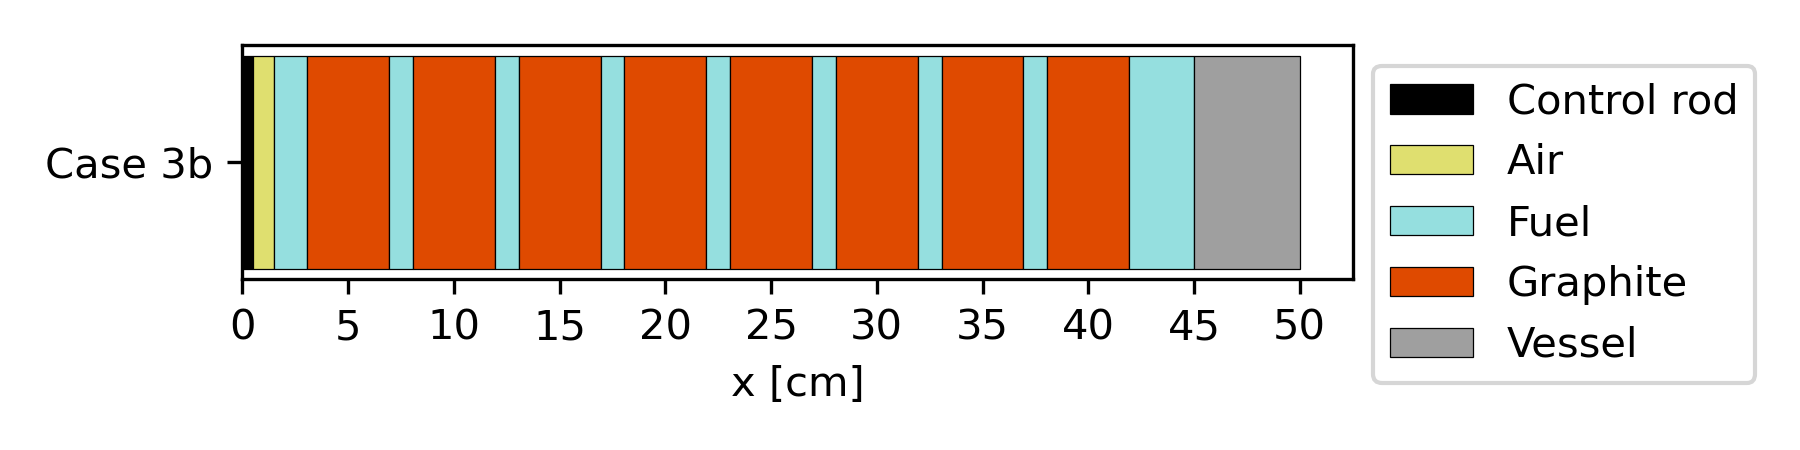
\includegraphics[width=.75\columnwidth]{case-3b-geometry}
	\caption{1-D geometry for Case 3b.}
	\label{fig:3b-geometry}
\end{figure}

Here, I use Case 3b of the 1-D test cases to be covered in Chapter \ref{chap:msre}
to illustrate the buffer region and the behavior of $\vec{D}_g$. Case 3b is a 1-D slab problem
consisting of control rod, air, fuel-graphite repeating lattice, and reactor vessel regions as
shown in Figure \ref{fig:3b-geometry}. The fuel regions are neutron-multiplying media containing
$^\text{235}$U fissile material. I took material compositions of each region from the \gls{MSRE}
reference design and the start-up fuel composition \cite{fratoni_molten_2020}.
Case 3b has reflecting boundary conditions on the left boundary and vacuum boundary conditions on
the right boundary.
%
\begin{figure}[htb!]
    \centering
    \begin{subfigure}[t]{.49\textwidth}
        \centering
        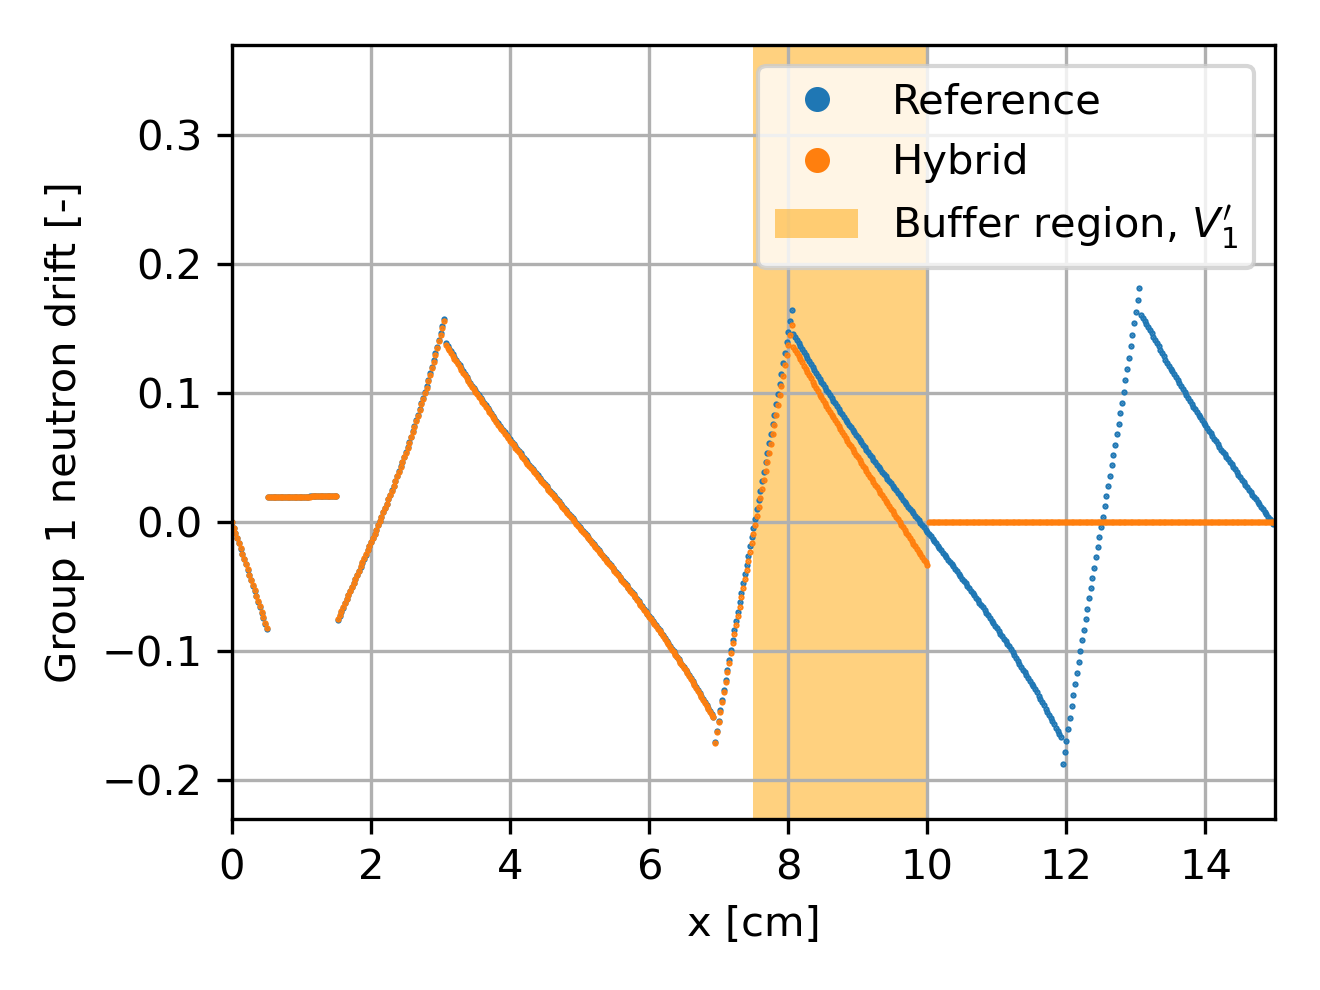
\includegraphics[width=\textwidth]{case-3b-group-1-drift}
    \end{subfigure}
    \hfill
    \begin{subfigure}[t]{.49\textwidth}
        \centering
        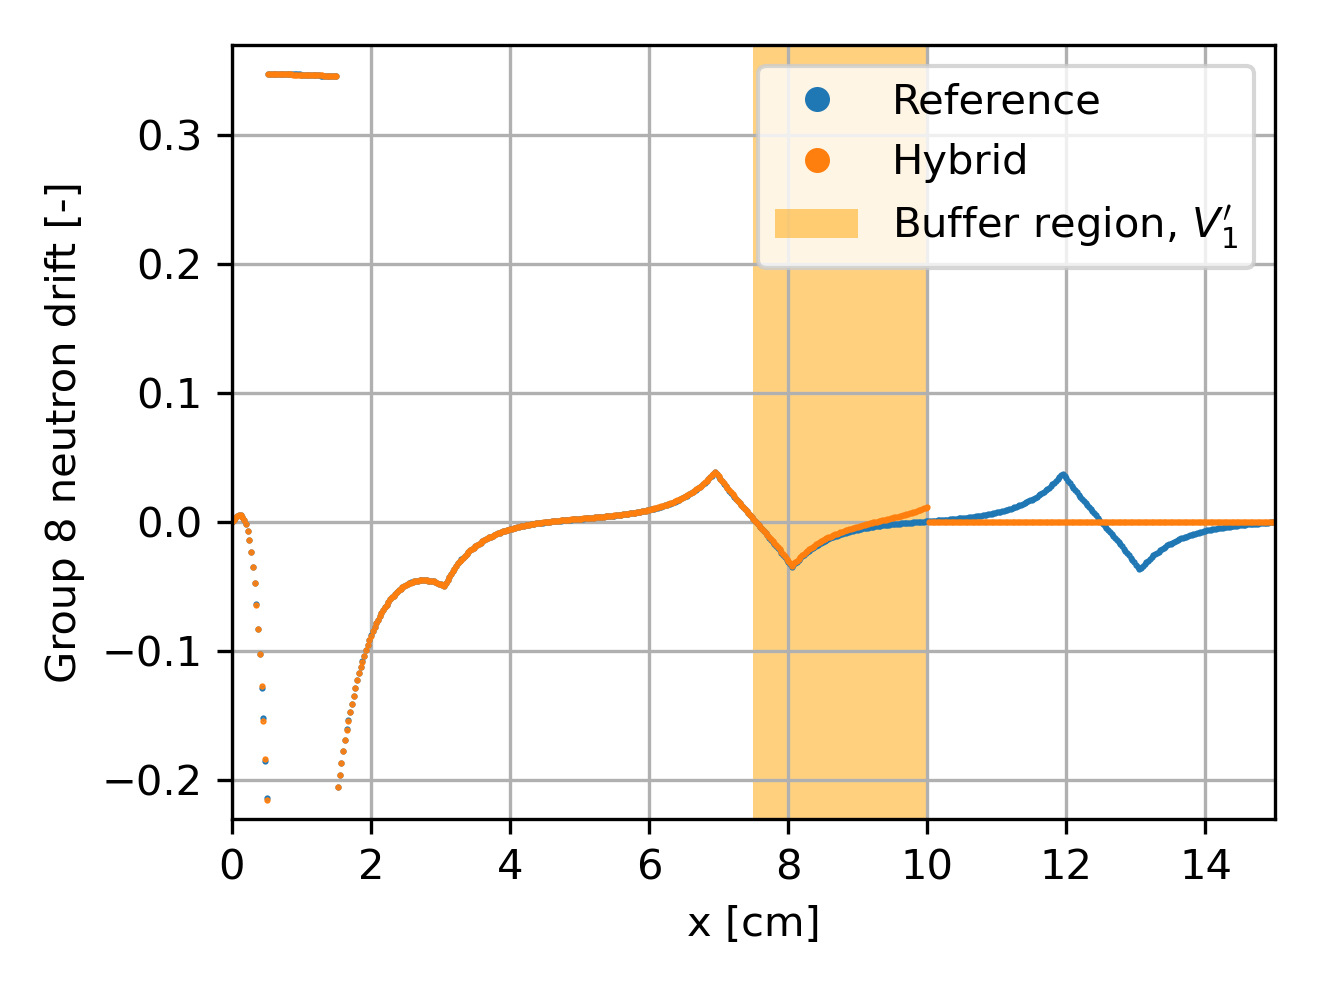
\includegraphics[width=\textwidth]{case-3b-group-8-drift}
    \end{subfigure}
    \caption{The reference and hybrid drift ($\vec{D}_g$) distributions for group 1 and 8 calculated
      from $S_8$ and $S_8$-diffusion simulations. The correction subregion $V_1$ spans $x=0$ cm to
      $x=10$ cm.}
    \label{fig:3b-drift}
\end{figure}

I ran an eight energy group $S_8$ $k$-eigenvalue simulation with the newly implemented $S_N$ solver
on Moltres to generate reference $\vec{D}_g$ distributions. I also ran an eight-group hybrid
$S_8$-diffusion simulation with the $S_8$ method for generating $\vec{D}_g$ in $V_1$. I set $V_1$
to encompass the control rod region and its vicinity from $x=0$ to $10$ cm based on the geometry in
Figure \ref{fig:3b-geometry}. Figure \ref{fig:3b-drift} shows the $\vec{D}_1$ and $\vec{D}_8$
distributions from $x=0$ to $15$ from the reference $S_8$ and hybrid simulations. The hybrid
$\vec{D}_g$ distribution is zero beyond $x=10$ cm because no corrections are generated outside of
$V_1$. Comparing the hybrid distributions to the reference distributions in both energy groups, the
hybrid distributions are accurate up to around $x=8$ cm. Working backward towards the control rod
at $x=0$-$0.5$ cm, the $\vec{D}_g$ values go to zero at $x=7.5$ cm. Therefore, the buffer
region $V_1'$ lies between $x=7.5$ cm and $x=10$ cm. While $V_1$ is pre-determined at the start of
the simulation and fixed for all energy groups, $V_1'$ does not necessarily coincide for all
energy groups and coordinate axes.

\section{Numerical Implementation}

In this section, I detail the numerical implementation of the hybrid $S_N$-diffusion method with
drift correction terms. As mentioned in Section \ref{sec:transport-correction}, I opted for the
drift correction terms over diffusion correction for investigations beyond 1-D test cases.
Therefore, for brevity, I moved numerical implementation details for the hybrid method with
diffusion correction to Appendix A.

In Section \ref{sec:moltres-description}, I detailed the code structure of Moltres
\cite{lindsay_moltres_2017} in relation to the underlying \gls{MOOSE} finite-element framework
\cite{giudicelli_30_2024} and the pre-existing multigroup neutron diffusion and thermal-hydraulics
models. I implemented the hybrid $S_N$-diffusion model in Moltres to
leverage existing capabilities and functions that are also relevant to the new $S_N$ neutron
transport model and the $S_N$-to-diffusion coupling features. I also leveraged several basic
functions from \gls{MOOSE} that are useful for setting up physics models.

All source code for the hybrid $S_N$-diffusion model is hosted on my Moltres GitHub fork
repository\footnote{\url{https://github.com/smpark7/moltres/tree/sn-method}} as of the time of
writing. This branch may be merged into the original upstream Moltres GitHub repository in the near
future.

Moltres presently comes with a Python script for parsing and extracting neutron group constant data
from OpenMC \cite{boyd_multigroup_2019} or Serpent 2 \cite{leppanen_serpent_2014} simulation
output files. The script reorganizes the group constant data into a
JSON format file. I expanded the Python script to extract
the macroscopic total cross sections $\Sigma_{t,g}$ and the higher-order macroscopic Legendre
scattering moments $\Sigma^{g'\rightarrow g}_{s,l}$ for the $S_N$ neutron transport model. A new
\texttt{Material} class called \texttt{MoltresSNMaterial} creates material
property variables for each group constant for the $S_N$ model to read during a neutronics
simulation. If the user provides group constant data at multiple reactor temperature states,
\texttt{MoltresSNMaterial} can interpolate the data to simulate temperature-dependent reactivity
changes.

The new \texttt{MoltresUtils} class contains ``utility'' functions required by the $S_N$ model.
These functions include: a function to retrieve directions and weights defined by a
level-symmetric quadrature set of order $N$, a function to retrieve reflecting directions at
reflecting boundaries, and a function to compute spherical harmonic flux moments for anisotropic
scattering. I pre-computed the direction and weight values for the level-symmetric quadrature sets
using a Python script and hard-coded them in Moltres to reduce computational burden during
simulations.

The \gls{SAAF} $S_N$ method defines $G$ energy groups and $N_d$ discrete directions for a total
of $G\times N_d$ angular flux variables $\Psi_{g,d}$. The Moltres $S_N$ model groups the
$\Psi_{g,d}$ variables by energy group into $G$ array variables. An array variable is a
set of standard field variables to help with dealing with setting up simulations with high
dimensionality. Each standard variable of an array variable is referred to as a component in the
array variable. In this work, I opted for
2nd-order Lagrange shape functions to approximate the $\Psi_{g,d}$ variables in the finite-element
analysis. The 2nd-order approximation showed better convergence rates in mesh refinement studies.

The terms in the \gls{SAAF} $S_N$ equations (Eqs.\ \ref{eq:time-derivative}-\ref{eq:reflecting-bc})
are represented by kernel and BC classes inheriting from \texttt{ArrayKernel} and
\texttt{ArrayIntegratedBC} template classes. Table \ref{tab:saaf-sn} lists the class names
corresponding to each term in Eq.\ \ref{eq:saaf-vt}.
%
\begin{table}[htb]
  \centering
  \caption{Names of the Kernels and BCs representing the \gls{SAAF} $S_N$ equations.}
  \begin{tabular}{l l l}
    \toprule
    Term name & Class name \\
    \midrule
    Time derivative & \texttt{SNTimeDerivative} \\
    Streaming & \texttt{SNStreaming} \\
    Collision & \texttt{SNCollision} \\
    Scattering & \texttt{SNScattering} \\
    Prompt fission source & \texttt{SNFission} \\
    Delayed neutron source & \texttt{SNDelayed} \\
    Vacuum boundary & \texttt{SNVacuumBC} \\
    Reflecting boundary & \texttt{SNReflectingBC} \\
    Hybrid method boundary source & \texttt{SNDiffusionBC} \\
    \bottomrule
  \end{tabular}
  \label{tab:saaf-sn}
\end{table}

The \gls{MOOSE} framework leverages the Eigen \cite{guennebaud_eigen_2010} C++ template library for
linear algebra operations defined in ArrayKernels and ArrayBCs for array variables. The \gls{SAAF}
$S_N$ kernels and BCs contain functions for computing the residual and Jacobian contributions of
each term. The \gls{FEM} numerical solver deems to have reached a converged solution if the sum of
residual contributions falls below a defined tolerance value. All $S_N$ simulations in this work
employ the \gls{PJFNK} method \cite{knoll_jacobian-free_2004} with HYPRE-BoomerAMG
\cite{hypre_hypre_2022} for preconditioning. BoomerAMG is a parallel implementation of the
algebraic multigrid method from the HYPRE linear solver library.

Moltres initializes the drift correction variables $\vec{D}_g$ as auxiliary array variables
with three components corresponding to their $x$, $y$, and $z$ components. Auxiliary variables
encompass all field variables which are not directly determined during the \gls{PJFNK}
calculation stage. The drift and boundary correction variables are computed during the
post-calculation stages using $\Psi_{g,d}$.
I created new kernel classes, \texttt{GroupDrift} and \texttt{VacuumCorrectionBC}, to add the
drift and boundary correction terms to the transport-corrected neutron diffusion solver.

I employed the \texttt{MultiApp} system \cite{gaston_physics-based_2015} to implement the fixed point
iterative coupling between the $S_N$ and neutron diffusion solvers for the hybrid $S_N$-diffusion method.
The \texttt{MultiApp} and \texttt{Transfers} systems from \gls{MOOSE} provide flexible interfaces
for setting up iterative solvers and transferring data between the solvers. A typical hybrid
method simulation on Moltres starts with the neutron diffusion solver for the first estimate of the
neutron flux distribution. Moltres transfers the neutron flux distribution to the $S_N$ solver to
compute the boundary source distribution. The $S_N$ solver then generates its own flux estimate and
computes drift and boundary correction variables for the neutron diffusion solver. Moltres
transfers the correction variables to the neutron diffusion solver to compute its next flux
estimate. This process iterates until the neutron flux distribution converges to within tolerance
values provided in the input file.

\section{Summary} \label{sec:hybrid-summary}

The hybrid $S_N$-diffusion method improves on the standard neutron
diffusion method by iteratively applying transport corrections generated from solving the $S_N$
neutron transport
method in subdomains containing highly neutron-absorbing regions (e.g., control rods). By limiting
the size of the subdomain in which $S_N$ subsolver is active, the hybrid method saves on
computational expense at the cost of some accuracy in the regions not treated with transport
corrections. In turn, the neutron diffusion subsolver provides approximate boundary source terms
for the $S_N$ subsolver boundary conditions. 

I presented two different formulations of transport correction that I investigated in this work for
implementation in the hybrid method: diffusion correction and drift correction. Diffusion
correction involves replacing the diffusion coefficient in the neutron diffusion equations with
corrected coefficients derived from neutron transport methods. Drift correction involves
introducing additional drift terms to the neutron diffusion equations to provide transport
corrections. I found drift correction to be more promising due to issues with division by zero when
obtaining diffusion corrections.

In my investigations with the hybrid method, I found that the $S_N$ subsolver produces
accurate transport correction values in most of the subdomain. However, the transport correction
values near the $S_N$ subsolver boundary are inaccurate due to the approximate boundary conditions
provided by the diffusion subsolver. Thus, I developed and presented a numerical fix for discarding
inaccurate transport correction values and preserving the smoothness of the neutron flux and flux
gradient solution.

By implementing the hybrid method in Moltres, I leveraged existing neutronics modelling
capabilities and parallel numerical solver libraries available through Moltres and \gls{MOOSE} to
enable full-core, time-dependent reactor simulations on \gls{HPC} clusters.
In the next chapter, I verify the hybrid method against Monte Carlo and $S_N$ neutron transport
methods through various neutronics test cases and discuss some significant observations made in my
investigations.
